\documentclass[]{article}
\usepackage{lmodern}
\usepackage{amssymb,amsmath}
\usepackage{ifxetex,ifluatex}
\usepackage{fixltx2e} % provides \textsubscript
\ifnum 0\ifxetex 1\fi\ifluatex 1\fi=0 % if pdftex
  \usepackage[T1]{fontenc}
  \usepackage[utf8]{inputenc}
\else % if luatex or xelatex
  \ifxetex
    \usepackage{mathspec}
  \else
    \usepackage{fontspec}
  \fi
  \defaultfontfeatures{Ligatures=TeX,Scale=MatchLowercase}
\fi
% use upquote if available, for straight quotes in verbatim environments
\IfFileExists{upquote.sty}{\usepackage{upquote}}{}
% use microtype if available
\IfFileExists{microtype.sty}{%
\usepackage{microtype}
\UseMicrotypeSet[protrusion]{basicmath} % disable protrusion for tt fonts
}{}
\usepackage[margin=1in]{geometry}
\usepackage{hyperref}
\hypersetup{unicode=true,
            pdftitle={R Notebook},
            pdfborder={0 0 0},
            breaklinks=true}
\urlstyle{same}  % don't use monospace font for urls
\usepackage{color}
\usepackage{fancyvrb}
\newcommand{\VerbBar}{|}
\newcommand{\VERB}{\Verb[commandchars=\\\{\}]}
\DefineVerbatimEnvironment{Highlighting}{Verbatim}{commandchars=\\\{\}}
% Add ',fontsize=\small' for more characters per line
\usepackage{framed}
\definecolor{shadecolor}{RGB}{248,248,248}
\newenvironment{Shaded}{\begin{snugshade}}{\end{snugshade}}
\newcommand{\AlertTok}[1]{\textcolor[rgb]{0.94,0.16,0.16}{#1}}
\newcommand{\AnnotationTok}[1]{\textcolor[rgb]{0.56,0.35,0.01}{\textbf{\textit{#1}}}}
\newcommand{\AttributeTok}[1]{\textcolor[rgb]{0.77,0.63,0.00}{#1}}
\newcommand{\BaseNTok}[1]{\textcolor[rgb]{0.00,0.00,0.81}{#1}}
\newcommand{\BuiltInTok}[1]{#1}
\newcommand{\CharTok}[1]{\textcolor[rgb]{0.31,0.60,0.02}{#1}}
\newcommand{\CommentTok}[1]{\textcolor[rgb]{0.56,0.35,0.01}{\textit{#1}}}
\newcommand{\CommentVarTok}[1]{\textcolor[rgb]{0.56,0.35,0.01}{\textbf{\textit{#1}}}}
\newcommand{\ConstantTok}[1]{\textcolor[rgb]{0.00,0.00,0.00}{#1}}
\newcommand{\ControlFlowTok}[1]{\textcolor[rgb]{0.13,0.29,0.53}{\textbf{#1}}}
\newcommand{\DataTypeTok}[1]{\textcolor[rgb]{0.13,0.29,0.53}{#1}}
\newcommand{\DecValTok}[1]{\textcolor[rgb]{0.00,0.00,0.81}{#1}}
\newcommand{\DocumentationTok}[1]{\textcolor[rgb]{0.56,0.35,0.01}{\textbf{\textit{#1}}}}
\newcommand{\ErrorTok}[1]{\textcolor[rgb]{0.64,0.00,0.00}{\textbf{#1}}}
\newcommand{\ExtensionTok}[1]{#1}
\newcommand{\FloatTok}[1]{\textcolor[rgb]{0.00,0.00,0.81}{#1}}
\newcommand{\FunctionTok}[1]{\textcolor[rgb]{0.00,0.00,0.00}{#1}}
\newcommand{\ImportTok}[1]{#1}
\newcommand{\InformationTok}[1]{\textcolor[rgb]{0.56,0.35,0.01}{\textbf{\textit{#1}}}}
\newcommand{\KeywordTok}[1]{\textcolor[rgb]{0.13,0.29,0.53}{\textbf{#1}}}
\newcommand{\NormalTok}[1]{#1}
\newcommand{\OperatorTok}[1]{\textcolor[rgb]{0.81,0.36,0.00}{\textbf{#1}}}
\newcommand{\OtherTok}[1]{\textcolor[rgb]{0.56,0.35,0.01}{#1}}
\newcommand{\PreprocessorTok}[1]{\textcolor[rgb]{0.56,0.35,0.01}{\textit{#1}}}
\newcommand{\RegionMarkerTok}[1]{#1}
\newcommand{\SpecialCharTok}[1]{\textcolor[rgb]{0.00,0.00,0.00}{#1}}
\newcommand{\SpecialStringTok}[1]{\textcolor[rgb]{0.31,0.60,0.02}{#1}}
\newcommand{\StringTok}[1]{\textcolor[rgb]{0.31,0.60,0.02}{#1}}
\newcommand{\VariableTok}[1]{\textcolor[rgb]{0.00,0.00,0.00}{#1}}
\newcommand{\VerbatimStringTok}[1]{\textcolor[rgb]{0.31,0.60,0.02}{#1}}
\newcommand{\WarningTok}[1]{\textcolor[rgb]{0.56,0.35,0.01}{\textbf{\textit{#1}}}}
\usepackage{graphicx,grffile}
\makeatletter
\def\maxwidth{\ifdim\Gin@nat@width>\linewidth\linewidth\else\Gin@nat@width\fi}
\def\maxheight{\ifdim\Gin@nat@height>\textheight\textheight\else\Gin@nat@height\fi}
\makeatother
% Scale images if necessary, so that they will not overflow the page
% margins by default, and it is still possible to overwrite the defaults
% using explicit options in \includegraphics[width, height, ...]{}
\setkeys{Gin}{width=\maxwidth,height=\maxheight,keepaspectratio}
\IfFileExists{parskip.sty}{%
\usepackage{parskip}
}{% else
\setlength{\parindent}{0pt}
\setlength{\parskip}{6pt plus 2pt minus 1pt}
}
\setlength{\emergencystretch}{3em}  % prevent overfull lines
\providecommand{\tightlist}{%
  \setlength{\itemsep}{0pt}\setlength{\parskip}{0pt}}
\setcounter{secnumdepth}{0}
% Redefines (sub)paragraphs to behave more like sections
\ifx\paragraph\undefined\else
\let\oldparagraph\paragraph
\renewcommand{\paragraph}[1]{\oldparagraph{#1}\mbox{}}
\fi
\ifx\subparagraph\undefined\else
\let\oldsubparagraph\subparagraph
\renewcommand{\subparagraph}[1]{\oldsubparagraph{#1}\mbox{}}
\fi

%%% Use protect on footnotes to avoid problems with footnotes in titles
\let\rmarkdownfootnote\footnote%
\def\footnote{\protect\rmarkdownfootnote}

%%% Change title format to be more compact
\usepackage{titling}

% Create subtitle command for use in maketitle
\providecommand{\subtitle}[1]{
  \posttitle{
    \begin{center}\large#1\end{center}
    }
}

\setlength{\droptitle}{-2em}

  \title{R Notebook}
    \pretitle{\vspace{\droptitle}\centering\huge}
  \posttitle{\par}
    \author{}
    \preauthor{}\postauthor{}
    \date{}
    \predate{}\postdate{}
  

\begin{document}
\maketitle

This is an \href{http://rmarkdown.rstudio.com}{R Markdown} Notebook.
When you execute code within the notebook, the results appear beneath
the code.

Try executing this chunk by clicking the \emph{Run} button within the
chunk or by placing your cursor inside it and pressing
\emph{Ctrl+Shift+Enter}.

\begin{Shaded}
\begin{Highlighting}[]
\FunctionTok{library}\NormalTok{(dplyr)}
\end{Highlighting}
\end{Shaded}

\begin{verbatim}
## 
## Attaching package: 'dplyr'
\end{verbatim}

\begin{verbatim}
## The following objects are masked from 'package:stats':
## 
##     filter, lag
\end{verbatim}

\begin{verbatim}
## The following objects are masked from 'package:base':
## 
##     intersect, setdiff, setequal, union
\end{verbatim}

\begin{Shaded}
\begin{Highlighting}[]
\FunctionTok{library}\NormalTok{(readxl)}
\FunctionTok{library}\NormalTok{(tidyr)}
\FunctionTok{library}\NormalTok{(moments)}
\end{Highlighting}
\end{Shaded}

\begin{Shaded}
\begin{Highlighting}[]
\NormalTok{df }\OtherTok{\textless{}{-}}\NormalTok{ readxl}\SpecialCharTok{::}\FunctionTok{read\_excel}\NormalTok{(}\StringTok{"Zad\_domowe\_nr\_1\_2023\_2024\_KCh.xlsx"}\NormalTok{)}
\end{Highlighting}
\end{Shaded}

\begin{Shaded}
\begin{Highlighting}[]
\FunctionTok{head}\NormalTok{(df,}\DecValTok{5}\NormalTok{)}
\end{Highlighting}
\end{Shaded}

\begin{verbatim}
## # A tibble: 5 x 2
##   Nr_obserwacji Masa_ptaka
##           <dbl>      <dbl>
## 1             1       3.32
## 2             2       3.33
## 3             3       3.49
## 4             4       3.61
## 5             5       3.11
\end{verbatim}

\begin{Shaded}
\begin{Highlighting}[]
\FunctionTok{glimpse}\NormalTok{(df)}
\end{Highlighting}
\end{Shaded}

\begin{verbatim}
## Observations: 50
## Variables: 2
## $ Nr_obserwacji <dbl> 1, 2, 3, 4, 5, 6, 7, 8, 9, 10, 11, 12, 13, 14, 1...
## $ Masa_ptaka    <dbl> 3.32, 3.33, 3.49, 3.61, 3.11, 3.21, 3.26, 3.98, ...
\end{verbatim}

\begin{Shaded}
\begin{Highlighting}[]
\NormalTok{df }\SpecialCharTok{\%\textgreater{}\%}
  \FunctionTok{summarize}\NormalTok{(}
    \AttributeTok{srednia\_masa =} \FunctionTok{mean}\NormalTok{(Masa\_ptaka),}
    \AttributeTok{wariancja\_masy =} \FunctionTok{var}\NormalTok{(Masa\_ptaka) }\SpecialCharTok{*}\NormalTok{ (}\FunctionTok{nrow}\NormalTok{(df) }\SpecialCharTok{{-}} \DecValTok{1}\NormalTok{) }\SpecialCharTok{*}\NormalTok{ (}\DecValTok{1} \SpecialCharTok{/} \FunctionTok{nrow}\NormalTok{(df)),}
    \AttributeTok{odch\_stand\_masy =} \FunctionTok{sd}\NormalTok{(Masa\_ptaka) }\SpecialCharTok{*}\NormalTok{ (}\FunctionTok{nrow}\NormalTok{(df) }\SpecialCharTok{{-}} \DecValTok{1}\NormalTok{) }\SpecialCharTok{*}\NormalTok{ (}\DecValTok{1} \SpecialCharTok{/} \FunctionTok{nrow}\NormalTok{(df)),}
    \AttributeTok{pierw\_kwart\_masy =} \FunctionTok{quantile}\NormalTok{(Masa\_ptaka, }\FloatTok{0.25}\NormalTok{),}
    \AttributeTok{mediana\_masy =} \FunctionTok{quantile}\NormalTok{(Masa\_ptaka, }\FloatTok{0.5}\NormalTok{), }
    \AttributeTok{trz\_kwart\_masy =} \FunctionTok{quantile}\NormalTok{(Masa\_ptaka, }\FloatTok{0.75}\NormalTok{) )}
\end{Highlighting}
\end{Shaded}

\begin{verbatim}
## # A tibble: 1 x 6
##   srednia_masa wariancja_masy odch_stand_masy pierw_kwart_masy mediana_masy
##          <dbl>          <dbl>           <dbl>            <dbl>        <dbl>
## 1         3.55         0.0819           0.283             3.32         3.52
## # ... with 1 more variable: trz_kwart_masy <dbl>
\end{verbatim}

\begin{Shaded}
\begin{Highlighting}[]
\NormalTok{calc\_skewness\_coeff }\OtherTok{\textless{}{-}} \ControlFlowTok{function}\NormalTok{(numbers) \{}
  
\NormalTok{  xbar }\OtherTok{\textless{}{-}} \FunctionTok{mean}\NormalTok{(numbers)}
\NormalTok{  n }\OtherTok{\textless{}{-}} \FunctionTok{length}\NormalTok{(numbers)}
\NormalTok{  stand\_dev }\OtherTok{\textless{}{-}} \FunctionTok{sd}\NormalTok{(numbers) }\SpecialCharTok{*}\NormalTok{ (n }\SpecialCharTok{{-}} \DecValTok{1}\NormalTok{) }\SpecialCharTok{/}\NormalTok{ n}
\NormalTok{  num }\OtherTok{\textless{}{-}}\NormalTok{ (}\DecValTok{1} \SpecialCharTok{/}\NormalTok{ n) }\SpecialCharTok{*} \FunctionTok{sum}\NormalTok{((numbers }\SpecialCharTok{{-}}\NormalTok{ xbar) }\SpecialCharTok{\^{}} \DecValTok{3}\NormalTok{)}
\NormalTok{  denom }\OtherTok{\textless{}{-}}\NormalTok{ stand\_dev }\SpecialCharTok{\^{}} \DecValTok{3}
\NormalTok{  skew }\OtherTok{\textless{}{-}}\NormalTok{ num }\SpecialCharTok{/}\NormalTok{ denom}
  
  \FunctionTok{return}\NormalTok{(skew)}
\NormalTok{\}}
\end{Highlighting}
\end{Shaded}

\begin{Shaded}
\begin{Highlighting}[]
\NormalTok{quartile\_coeff\_of\_dispersion }\OtherTok{\textless{}{-}} \ControlFlowTok{function}\NormalTok{(numbers) \{}
  
\NormalTok{  first.quart }\OtherTok{\textless{}{-}} \FunctionTok{quantile}\NormalTok{(numbers, }\FloatTok{0.25}\NormalTok{, }\AttributeTok{names =} \ConstantTok{FALSE}\NormalTok{)}
\NormalTok{  third.quart }\OtherTok{\textless{}{-}} \FunctionTok{quantile}\NormalTok{(numbers, }\FloatTok{0.75}\NormalTok{, }\AttributeTok{names =} \ConstantTok{FALSE}\NormalTok{)}
  
\NormalTok{  numerator }\OtherTok{=}\NormalTok{ third.quart }\SpecialCharTok{{-}}\NormalTok{ first.quart}
\NormalTok{  denominator }\OtherTok{=}\NormalTok{ third.quart }\SpecialCharTok{+}\NormalTok{ first.quart}
  
\NormalTok{  quartile.dispersion }\OtherTok{=}\NormalTok{ numerator }\SpecialCharTok{/}\NormalTok{ denominator}
  
  \FunctionTok{return}\NormalTok{(quartile.dispersion)}
\NormalTok{\}}
\end{Highlighting}
\end{Shaded}

\begin{Shaded}
\begin{Highlighting}[]
\FunctionTok{quartile\_coeff\_of\_dispersion}\NormalTok{(df}\SpecialCharTok{$}\NormalTok{Masa\_ptaka)}
\end{Highlighting}
\end{Shaded}

\begin{verbatim}
## [1] 0.06445932
\end{verbatim}

\begin{Shaded}
\begin{Highlighting}[]
\NormalTok{df }\SpecialCharTok{\%\textgreater{}\%}
  \FunctionTok{summarize}\NormalTok{(}
    \AttributeTok{rozstep\_miedzykwartylowy =} \FunctionTok{IQR}\NormalTok{(Masa\_ptaka), }
    \AttributeTok{odch\_cwiartkowe =} \FunctionTok{IQR}\NormalTok{(Masa\_ptaka) }\SpecialCharTok{/} \DecValTok{2}\NormalTok{,}
    \AttributeTok{skosnosc =} \FunctionTok{skewness}\NormalTok{(Masa\_ptaka),}
    \AttributeTok{pozycyjna\_skosnosc =} \FunctionTok{quartile\_coeff\_of\_dispersion}\NormalTok{(Masa\_ptaka),}
    \AttributeTok{kurtoza=}\FunctionTok{kurtosis}\NormalTok{(Masa\_ptaka)}
    
\NormalTok{  )}
\end{Highlighting}
\end{Shaded}

\begin{verbatim}
## # A tibble: 1 x 5
##   rozstep_miedzykwartyl~ odch_cwiartkowe skosnosc pozycyjna_skosno~ kurtoza
##                    <dbl>           <dbl>    <dbl>             <dbl>   <dbl>
## 1                  0.458           0.229    0.122            0.0645    2.21
\end{verbatim}

\begin{Shaded}
\begin{Highlighting}[]
\FunctionTok{calc\_skewness\_coeff}\NormalTok{(df}\SpecialCharTok{$}\NormalTok{Masa\_ptaka)}
\end{Highlighting}
\end{Shaded}

\begin{verbatim}
## [1] 0.1261247
\end{verbatim}

\begin{Shaded}
\begin{Highlighting}[]
\FunctionTok{skewness}\NormalTok{(df}\SpecialCharTok{$}\NormalTok{Masa\_ptaka)}
\end{Highlighting}
\end{Shaded}

\begin{verbatim}
## [1] 0.12236
\end{verbatim}

\begin{Shaded}
\begin{Highlighting}[]
\FunctionTok{boxplot}\NormalTok{(df}\SpecialCharTok{$}\NormalTok{Masa\_ptaka, }\AttributeTok{range =} \DecValTok{0}\NormalTok{, }\AttributeTok{main =} \StringTok{"Rozkład mas ptaków"}\NormalTok{, }\AttributeTok{ylab =} \StringTok{\textquotesingle{}Masa ptaka {-} funty\textquotesingle{}}\NormalTok{)}
\end{Highlighting}
\end{Shaded}

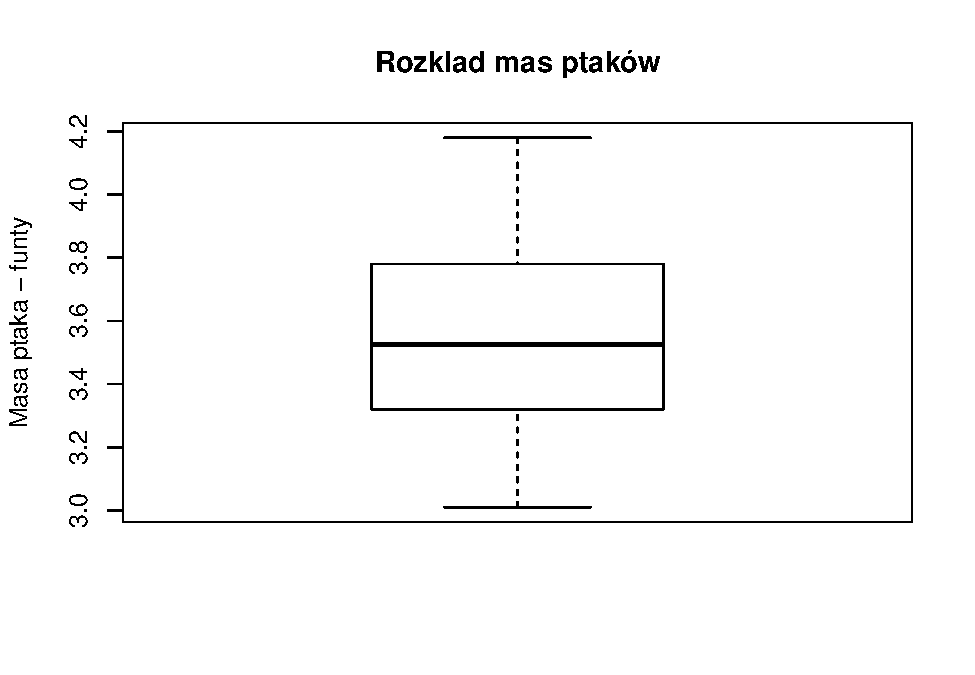
\includegraphics{proj_one_new_notebook_files/figure-latex/unnamed-chunk-12-1.pdf}
Brak obserwacji odstających.

\begin{Shaded}
\begin{Highlighting}[]
\FunctionTok{max}\NormalTok{(df}\SpecialCharTok{$}\NormalTok{Masa\_ptaka)}
\end{Highlighting}
\end{Shaded}

\begin{verbatim}
## [1] 4.18
\end{verbatim}

\begin{Shaded}
\begin{Highlighting}[]
\FunctionTok{min}\NormalTok{(df}\SpecialCharTok{$}\NormalTok{Masa\_ptaka)}
\end{Highlighting}
\end{Shaded}

\begin{verbatim}
## [1] 3.01
\end{verbatim}

\begin{Shaded}
\begin{Highlighting}[]
\FunctionTok{hist}\NormalTok{(df}\SpecialCharTok{$}\NormalTok{Masa\_ptaka, }\AttributeTok{main =} \StringTok{"Rozkład mas ptaków"}\NormalTok{, }\AttributeTok{xlab =} \StringTok{\textquotesingle{}Masa ptaka {-} funty\textquotesingle{}}\NormalTok{, }\AttributeTok{ylab=}\StringTok{"Częstość"}\NormalTok{)}
\end{Highlighting}
\end{Shaded}

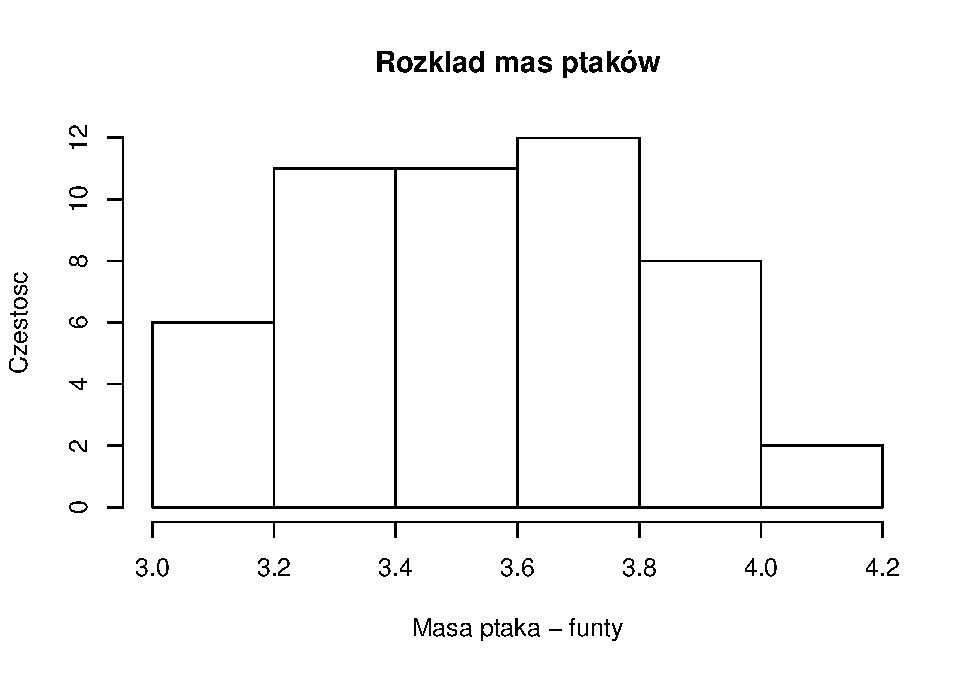
\includegraphics{proj_one_new_notebook_files/figure-latex/unnamed-chunk-15-1.pdf}


\end{document}
